\clearpage

\section{Simplified Coherent Receiver}

\begin{tcolorbox}	
\begin{tabular}{p{2.75cm} p{0.2cm} p{10.5cm}} 	
\textbf{Student Name}  &:& Romil Patel\\
\textbf{Starting Date} &:& August 16, 2017\\
\textbf{Goal}          &:& Develop a simplified structure (low cost) for a coherent receiver, that can be used in coherent PON, inter-data center connections, or metropolitan networks (optical path lengths should be < 100 km).
\end{tabular}
\end{tcolorbox}

In recent days, homodyne detection has been discussed and investigated a lot due to the advancement in the DSP in the electrical domain. However, a major drawback of homodyne detection is the incoming signal should be separated into inphase and quadrature (I/Q) signals in the optical domain. Therefore, it demands more hardware to accommodate the requirement of the signal separation  in the optical domain. For instance, 4 balanced photodetectors with double hybrid structures and 4-channel ADCs are required.
On the other hand, heterodyne receiver simplifies the detection scheme to some extent with the requirement of having only half of photodetectors and ADC.\\
Such coherent detection scheme constitute the solution for the medium-to-long-reach application; however, the cost of coherent receiver becomes a major obstacle in the case of short-reach links applications like PON, inter-data-center communications, metropolitan network etc. In order to get rid of higher cost and to make the transceiver more efficiently applicable in short-reach links, a new architecture of optical receiver has been proposed which combines the advantages of coherent transmission and cost effectiveness of direct detection. The working principle of the receiver is based on the famous Kramers-Kronig(KK) relationship. It facilitates digital post-compensation of linear propagation impairments which is highly efficient in terms of spectral occupancy and energy consumptions.

\begin{figure}[h]
	\centering
	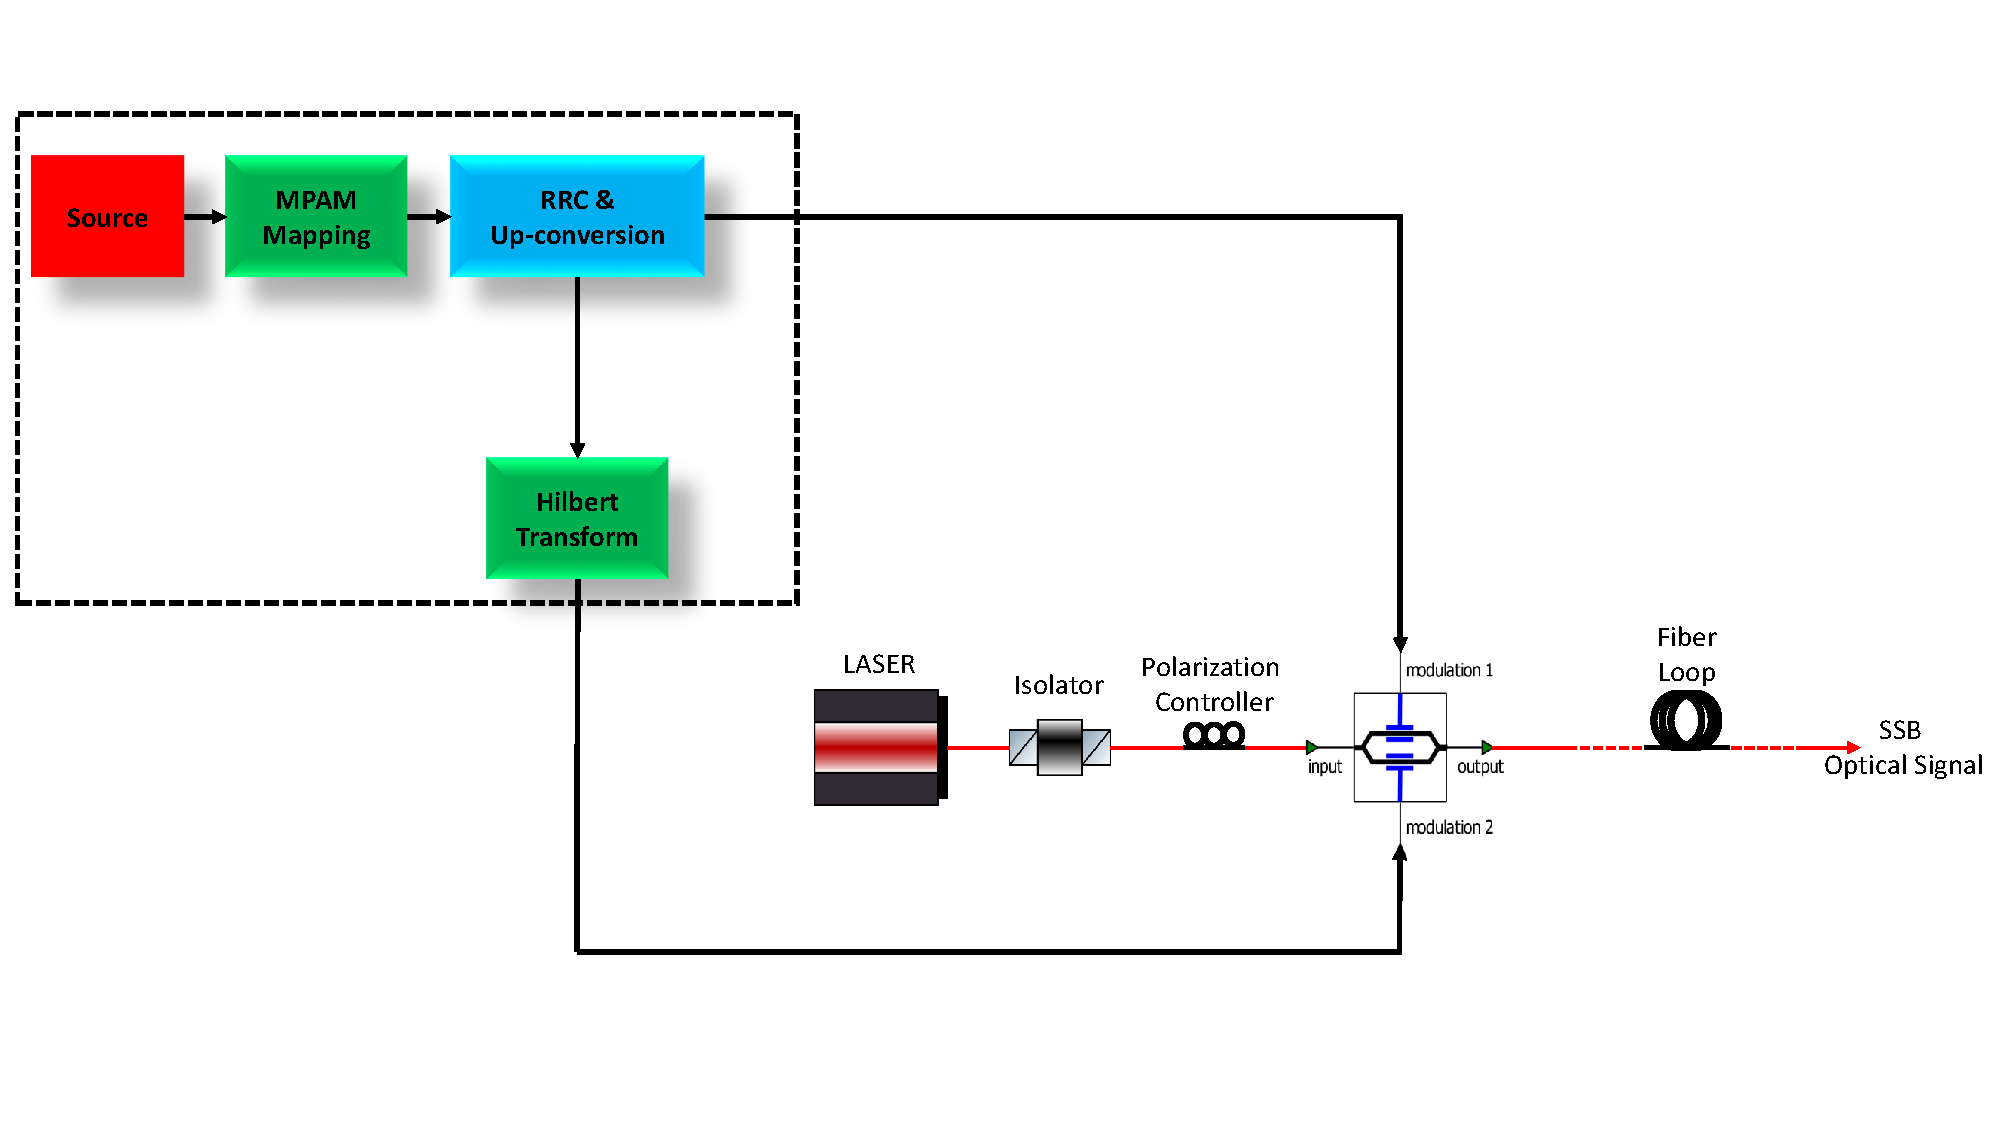
\includegraphics[width=1.0\textwidth, height=7cm]{./sdf/simplified_coherent_receiver/figures/Single_Polarization_Tx.pdf}
	\caption{Simplified Coherent Transceiver}\label{simplified_coherent_transceiver}
\end{figure}

\begin{figure}[h]
	\centering
	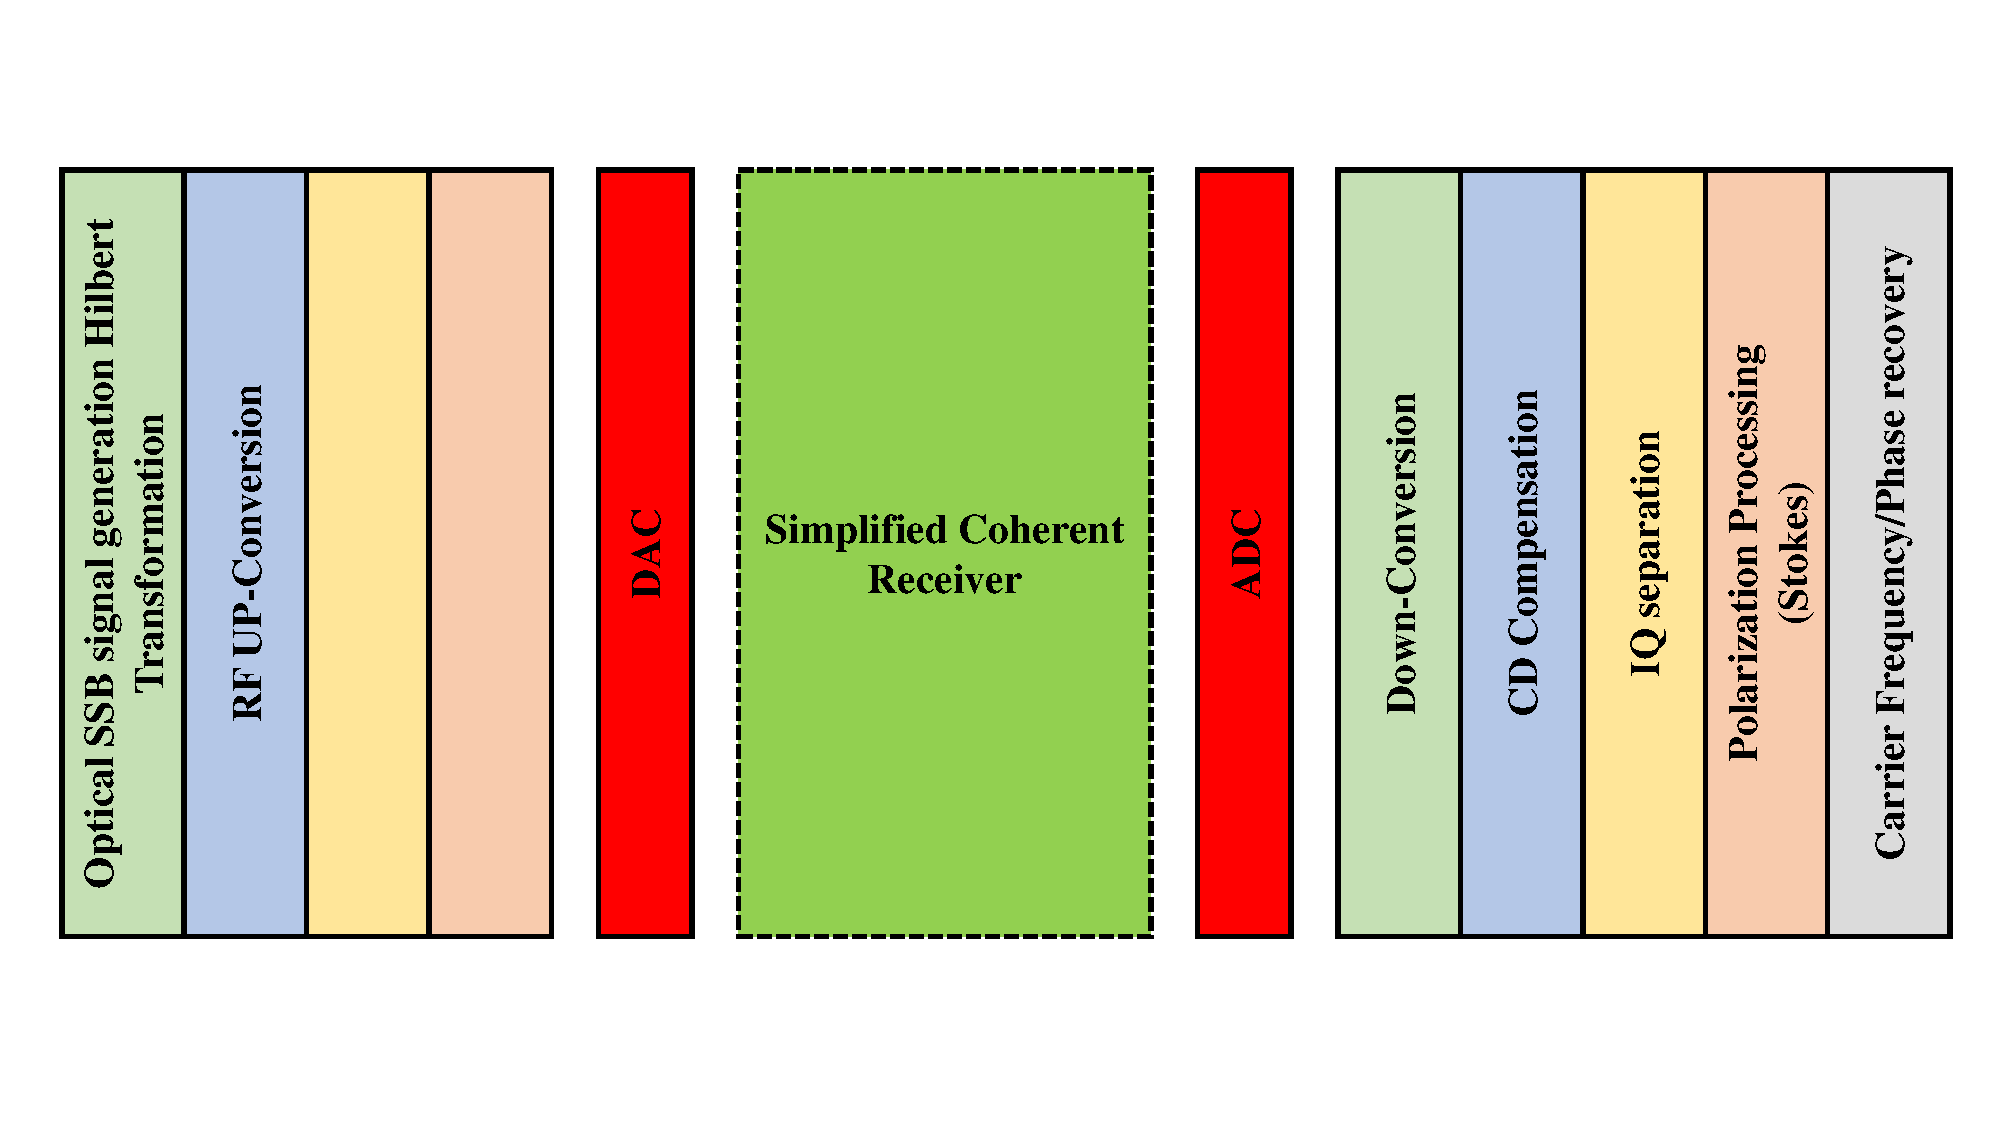
\includegraphics[width=1.0\textwidth, height=8cm]{./sdf/simplified_coherent_receiver/figures/detailed_subsystem.pdf}
	\caption{Tx/Rx DSP main subsystem}\label{DSP_main_subsystem}
\end{figure}

\subsection{Tx side}
Dual polarization(DP) DP-QPSK/DP-16QAM signals (1.25 Gbaud) to be generated at the Tx through an IQ modulator (Figure \ref{DSP_main_subsystem}) driven by DAC mounted in a FPGA. Polarization-division multiplexing is emulated by dividing the signal in two signals using an optical splitter, where a delay of 12 symbols is applied in order to decorrelate the two polarization tributaries and then, both signals are joined orthogonally employing a polarization beam combiner (PBC).

\subsection{Rx side}
At the receiver side, signal is coherently detected using a simplified coherent receiver and a local oscillator. The optical signal is then converted into the electrical domain using two balanced photodetector (BPD), or alternatively four photodetector, and amplified by a transimpedance amplifier (TIA). Following that, the signals are sampled by two 8-bit 2.5 GSa/s ADC and the this digitized signal sent to the FPGA (Virtex-7) where all post-detection DSP implemented in real-time.

